\section{Experimental setup}

\subsection{Dataset and its Challenges}

We use the dataset from the SemEval-2025 Task 10, Subtask 2, a task focused on multilingual propaganda narrative detection \cite{semeval2025task10}. While the full dataset spans five languages, our experiments focus on the English subset. A systematic analysis of the data reveals several key characteristics that motivate our architectural choices.

First, the dataset is fundamentally multi-label in nature. A majority of documents (54.0\%) are assigned more than one narrative, with an average of 2.28 labels per document. This necessitates a multi-label modeling approach.

Second, and most critically, the dataset exhibits a severe class imbalance. As shown in Figure~\ref{fig:narrative_distribution}, the 22 narrative labels follow a classic long-tailed distribution. The most frequent narrative appears 65 times more often than the least frequent one. This sparsity poses a significant challenge for traditional supervised models, which risk overfitting on the few ``head'' classes and failing to generalize to the many rare but meaningful ``tail'' classes. This characteristic strongly motivates our adoption of a zero-shot paradigm, which does not depend on label frequencies in a training set.

\begin{figure*}[!ht]
\centering
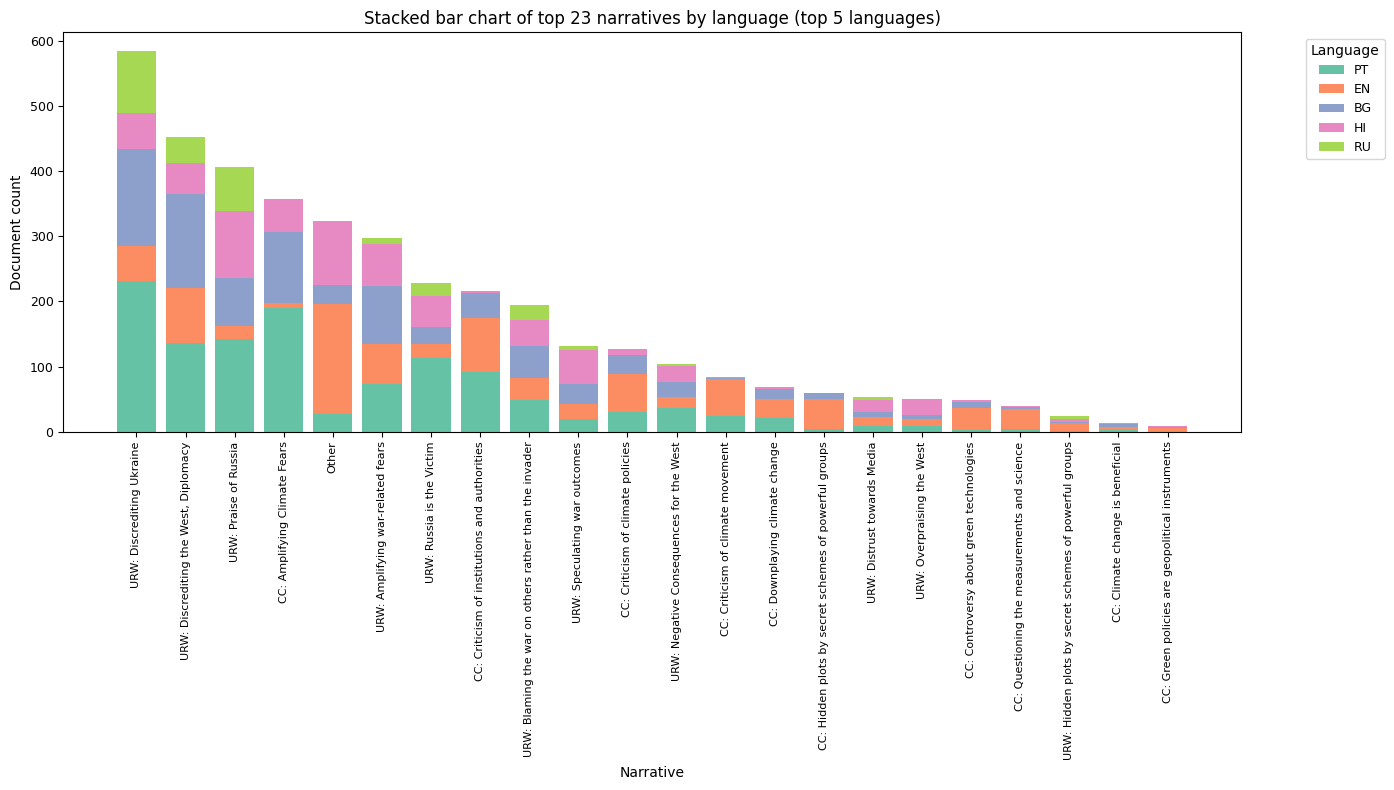
\includegraphics[width=0.95\textwidth]{assets/images/data_description/narrative_distribution.png}
\caption{Long-tailed distribution of narrative labels. A small number of frequent narratives dominate the dataset, while most are rare. This severe imbalance justifies the use of zero-shot LLM approaches that do not rely on large per-class training counts.}
\label{fig:narrative_distribution}
\end{figure*}

\subsection{System Configurations}

To isolate the contributions of our different architectural choices, we define and compare three distinct zero-shot systems. All systems are implemented using the LangGraph framework \cite{langgraph2024} and share the same foundational prompts to ensure a fair comparison.

\begin{enumerate}
\item \textbf{Naive Baseline (Single-Pass Actor):}
This configuration represents the most straightforward application of an LLM to the HMLC task. It consists of a single "Actor" agent that performs the classification for each hierarchical level. The output from the agent's first and only pass is taken as the final result. This system serves as our baseline to measure the performance of a standard, non-revising, and non-ensembled LLM classifier. For this configuration, we used gpt-5-nano as the LLM.

\item \textbf{Actor-Critic Pipeline:}
This system represents our initial effort to improve reliability through self-refinement. It extends the Naive Baseline by adding a "Critic" agent that reviews and validates the Actor's output. If the Critic identifies a flaw, it provides feedback, and the Actor makes a second, revised attempt. This configuration allows us to measure the impact of a single, iterative correction loop. The Actor and Critic agents were both implemented using gpt-5-nano.

\item \textbf{Agora (Multi-Agent Ensemble):}
This is our proposed framework, designed to achieve robustness through consensus. Instead of refinement, Agora employs a multi-agent ensemble where independent agents classify the text in parallel. Their outputs are then aggregated using a Majority Vote mechanism to determine the final label set. This configuration tests our primary hypothesis that consensus from multiple agents is more effective than the single-agent refinement loop. All agents in the Agora ensemble were implemented using gpt-5-nano.
\end{enumerate}

\subsection{Hardware Configuration}

All experiments were conducted on a machine with the following specifications:
\begin{itemize}
\item \textbf{Processor:} Intel Core 9 Ultra
\item \textbf{GPU:} NVIDIA RTX 4070 (8GB VRAM)
\item \textbf{Memory:} 32GB RAM
\item \textbf{Storage:} 1TB SSD
\end{itemize}

\subsection{Evaluation Scope}

We primarily evaluate the performance of our models on the English test set, providing detailed analysis and interpretation of the results on this language. However, to assess the multilingual capabilities of our approaches, we also conducted experiments on additional languages to validate the generalizability of our methods across different linguistic contexts.